\onehalfspacing

\section{Einleitung}
In diesem Kapitel wird neben der Motivation, Zielsetzung und Methodik dieser Arbeit auch auf das betriebliche Umfeld eingegangen. Dabei wird die Unternehmensstruktur erläutert, um den Lesenden einen besseren Überblick über die Aufgabenbereiche sowie Organisation des Projektumfeld zu ermöglichen. 
		\subsection{SICK}
		Die SICK AG mit Sitz in Waldkirch wurde 1946 durch Dr. E.h. Erwin Sick gegründet. Durch 		seine innovativ ausgeprägte Denkweise gelang ihm sechs Jahre später mit der Vorstellung 		seines Unfallschutz-Lichtvorhangs, auf der internationalen Werkzeugmaschinenmesse in 			Hannover, ein wirtschaftlicher Durchbruch \cite{SICK.2021}. Heute ist SICK einer der weltweit 				führenden Hersteller von Sensoren und Sensorlösungen in den Bereichen Logistik-, 				Fabrik-, und Prozessautomation. Der jährliche Umsatz des Unternehmens beläuft sich auf 			rund 1,7 Mrd. Euro. Aktuell werden weltweit rund 10.000 Mitarbeiter in fast 50 					Tochtergesellschaften beschäftigt.\cite{SICKAG.2020}
		Um als Globales Unternehmen bestehen zu können, ist die SICK AG organisatorisch in  SSU´s, GIC´s, GBC´s, Corporate Departments und Corporate Units gegliedert.
	\begin{figure}[h]
        \centering
        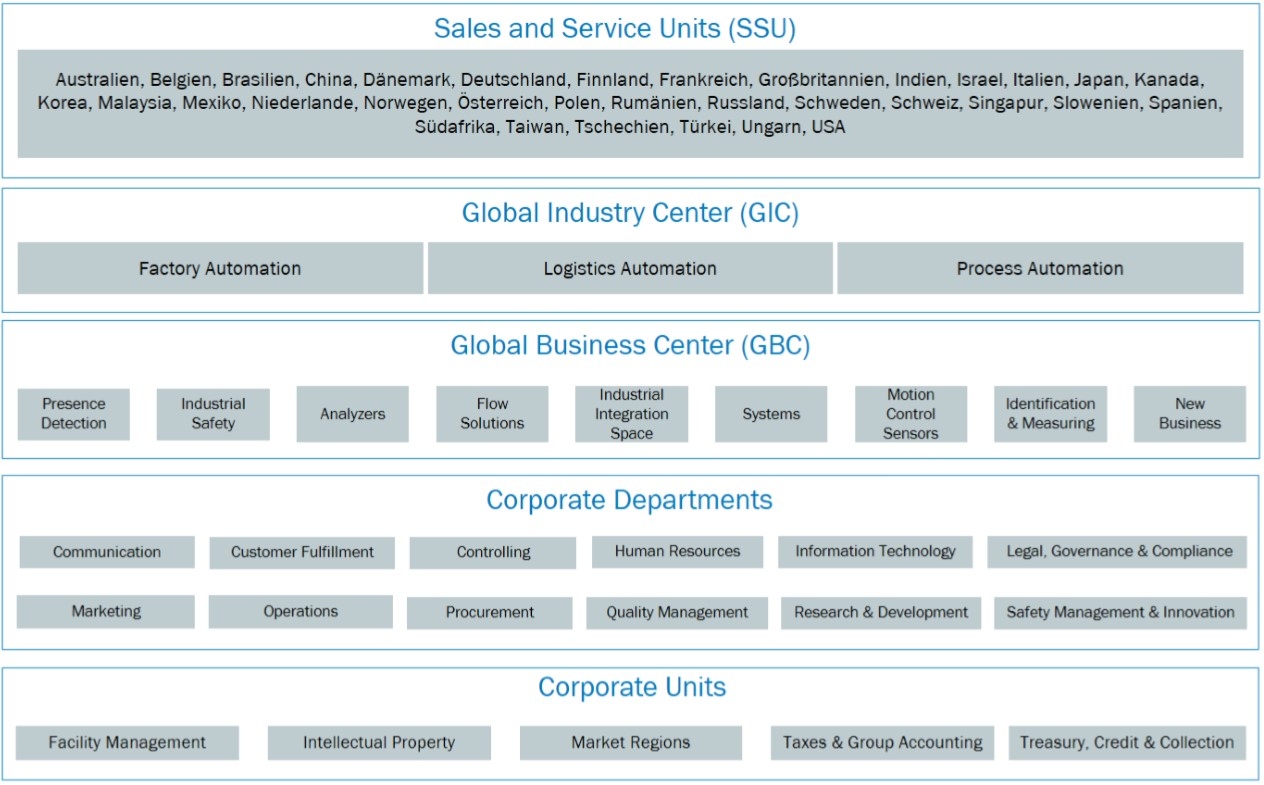
\includegraphics[width=1\textwidth]{img/OrganigramSick.jpg} 
        \caption[Unternehmensstruktur]{Unternehmensstruktur \cite{SICKAG.2020}}
        \label{fig:OrganigramSick.jpg}
    \end{figure}
Jedem Global Business Center (GBC) ist eine spezifische Produktsparte zugeordnet, welche durch die GBC betreut wird. Hierbei liegt der Fokus auf der Entwicklung und Produktion der in der Sparte angesiedelten Produkte. Die Sales and Service Units (SSU) betreuen den Vertrieb der in den GBC´s gefertigten Produkte. Ein Global Industry Center (GIC) bietet branchenspezifische Gesamtlösungen. Coporate Departments und Corporate Units werden auch als Zentralbereiche bezeichnet. Sie sind GBC übergreifend für alles zuständig was nicht direkt mit Entwicklung, Produktion und Vertrieb in Verbindung steht. Die Organisationsstruktur ist in der Abbildung \dq \nameref{fig:OrganigramSick.jpg}\dq~dargestellt.
		\subsection{SICK STEGMANN GmbH}
		Die Firma STEGMANN GmbH mit Standort in Donaueschingen wurde 1956 von Max Stegmann gegründet. Ihr Produktportfolio bestand zu Beginn hauptsächlich aus Kleinmotoren, Getrieben, Programmsteuerungen und feinmechanischen Baugruppen. 1960 wurde der erste inkrementelle Encoder entwickelt. 2002 wurde Stegmann durch die SICK AG aufgekauft und als Tochtergesellschaft in das Unternehmen eingegliedert.
Die SICK STEGMANN GmbH (GBC 07) gliedert sich in drei Business Center. 
Die BU71 ist zuständig für Motor Feedback Systeme, BU72 für Encoder und Neigungssensoren und die BU73 für Linear Encoder.\cite{SICKAG.2020}
		\subsection{Hardeware / CCE Team}
		Das Team Hardeware und \ac{CCE} ist Bestandteil der BU71. Das Hardeware Team beschäftigt sich vorwiegend mit der Entwicklung der für \ac{MFB} benötigten Hardware Komponenten. \ac{CCE} steht für Continuous and Customised Engineering. Das Team befasst sich mit der Anpassung von Bestandsprodukten nach kundenspezifischen Anforderungen sowie der Anpassung von Bestandsprodukten, zum Beispiel bei der Änderung eines Bauteils oder kleineren Anpassungen der Firmware.
	\subsection{Problemstellung}
	Der SKS bzw. SKM ist ein Motorfeedbacksystem, welches bereits seit mehreren Jahren durch die SICK STEGMANN GmbH vertrieben wird. Trotz der langen Lebenszeit des Produktes ist es immer noch eines der Absatz stärksten \ac{MFB} im Portfolio von SICK. Innerhalb des Gerätes dient ein ST7 Mikrocontroller als Recheneinheit. Dieser stellt u. a. die Kommunikation via Hiperface bereit. Der ST7 ist ein 8bit Mikrocontroller der Firma STMicroelektronics, welcher auf einer Von-Neumann-Architektur basiert\cite{mikrocontroller.net.2009}. ST hat bekannt gegeben, dass der ST7 in naher Zukunft das End of life erreicht und somit keine neuen ST7 mehr verfügbar sein werden. Aus diesem Grund ist SICK gezwungen eine Umstellung von ST7 auf den Nachfolger ST8 vorzunehmen. Im Rahmen der Umstellung muss eine Portierung der \ac{MFB} Software stattfinden. Im Zuge der Softwareportierung wird es zu einem erhöhten Testaufwand für das Produkt kommen. Da neben dem SKS bzw. SKM in Zukunft auch noch weitere \ac{MFB} portiert werden müssen, ergibt sich die Notwendigkeit einer universell einsetzbaren Testsuite, welche die Kernfunktionalitäten der Software im Rahmen des Automated Testing @ GBC07 Umfeldes abprüfen kann. 
	\subsection{Zielsetzung}
	Das Ziel der Arbeit ist die Entwickelung, sowie prototypische Implementierung einer universellen Testsuite. Die Testsuite soll so gestaltet werden, dass sie die Kernfunktionalitäten des Controllers, wie zum Beispiel die Kommunikation über das Hiperface Protokoll abdeckt. Diese Kernfunktionalitäten werden auch von anderen Produkten genutzt. Ziel ist es bei der späteren Portierung des Controllers und den damit verbundenen Tests, auf die Testsuite zurückgreifen zu können und mithilfe der darin vorhandenen Testfälle den Validierungsprozess zu beschleunigen. Weiterhin soll die Testsuite so gestaltet werden, dass sie auch für später folgende weitere Portierungen von ähnlichen Drehgebern verwendet werden kann.
	\subsection{Vorgehensweise}
	Zu Beginn des Projektes wird ein Überblick über die verschiedenen Themenbereiche (Hiperface Schnittstelle, \ac{MFB}, Automated-Testing etc.) geschaffen, sowie eine Projektplanung vorgenommen. Die Projektplanung umfasst hierbei u.a. die Zeitplanung. Aufgrund der Kürze des Projektes wurde hierbei auf eine Wochenplanung gesetzt. Die Planung sieht fünf Projektphasen vor (Einarbeitung, Analyse und Konzeption, Implementierung und Verifikation). Besonderes Augenmerk wird auf die Konzeptionsphase gelegt. Im Rahmen der Einarbeitungsphase werden die bereits existierenden Projekte betrachtet und eine Literaturrecherche durchgeführt. In der Analysephase werden die Testfälle anderer Produkte analysiert. Weiterhin wird geprüft, welche Testfälle ggf. übernommen werden können. In der Konzeptionsphase wird der Aufbau der Suite sowie die konkreten Testfälle definiert. Hierbei spielt die Planung der Softwarearchitektur eine große Rolle, da diese als Grundlage für den Erfolg des Projekt dient. Die Architektur soll hierbei auch später noch offen für Erweiterungen sein. In diesem Projektschritt kann teilweise auf vorhandenen Quellcode zurückgegriffen und dieser ggf. wiederverwendet werden. Die Implementierung erfolgt als proof of concept, da zum voraussichtlichen Ende des Projektes die Portierung noch nicht abgeschlossen sein wird. Um das Ergebnis des Projekts zu Verifizieren findet am Ende ein Abgleich mit den definierten Anforderungen statt. 
